\documentclass[12pt,a4paper]{article}
\usepackage[utf8]{inputenc}
\usepackage[spanish]{babel}
\usepackage{amsmath}
\usepackage{amsfonts}
\usepackage{amssymb}
\usepackage{makeidx}
\usepackage{graphicx}
\usepackage{lmodern}
\usepackage{kpfonts}
\usepackage{apacite}
\usepackage{multirow}
\usepackage{graphicx}
\setlength{\parindent}{0em}
\usepackage[left=3cm,right=3cm,top=2cm,bottom=2cm]{geometry}
\author{Pablo Vivas Corrales\footnote{\textit{Maestría Académica en Estadística. Universidad de Costa Rica}}\\\textit{pablo.vivas@ucr.ac.cr}}
\title{Análisis espacial del dengue en Costa Rica}
\date{16 de diciembre de 2019}
\begin{document}
\maketitle
\begin{abstract}
\noindent
La posición geográfica de Costa Rica posibilita al vector \textit{Aedes} la propagación de la enfermedad conocida como dengue. Solo en el año 2019 la sección de vigilancia del Ministerio de Salud reportó más de 8000 mil casos de esta enfermedad, siendo el cantón de Sarapiquí de Heredia un valor extremo (1816 casos registrados). Con esos datos e información obtenida del Instituo Nacional de Estadistica y Censos (INEC) se realizó un análisis espacial con los siguientes objetivos: (1) identificar la existencia de agrupaciones espaciales en los cantones de Costa Rica (2) determinar indicadores que están asociados con la aparición del dengue y (3) calcular el riesgo que tienen los habitantes de los cantones costarricenses de tener esta enfermedad. Se hace uso de la prueba I de Moran para contrastar la hipótesis de autocorrelación espacial. Asimismo se ajusta un modelo lineal, dos modelos autoregresivos (\textit{SAR \& CAR}) y un modelo lineal generalizado con un término no paramétrico, siendo este último el que posee un $R^{2}$ más elevado (93\%). Se utilizan técnicas propias del análisis epidemiológico, como el mapa de probabilidades de Choynowski y el cálculo de riesgos relativos, donde resultan significativos los cantones de: Sarapiquí, Guácimo, La Cruz, Turrialba, Atnas, Montes de Oro, Garabito \& Pococí. Se concluye con un análisis empírico bayesiano.\\
\textbf{Palabras clave:} \textit{Dengue, Análisis espacial, Modelos Autoregresivos \& Análisis Epidemiológico} 
\end{abstract}
\section{Introducción}

El dengue es una enfermedad viral transmitida por mosquitos que se ha propagado rápidamente en todas las regiones de la Organización Mundial de la Salud (OMS) en los últimos años. El virus del dengue es transmitido por mosquitos hembras, principalmente de la especie \textit{Aedes aegypti}. Este mosquito también es vector de virus como chikungunya, fiebre amarilla y zika. El dengue está muy extendido en las regiones tropicales y subtropicales \cite{OMS}. La incidencia del dengue ha crecido dramáticamente en todo el mundo en las últimas décadas. La gran mayoría de los casos son leves y autogestionados, y por lo tanto, el número real de casos de dengue no se informa. Muchos casos también se diagnostican erróneamente como otras enfermedades febriles \cite{Waggoner2016}.\\
\newline
El virus es altamente transmisible cuando la infestación por el vector es alta, lo que puede producir epidemias de dengue con alta morbilidad y mortalidad, en su forma grave. La infección que produce resulta en un amplio espectro de presentaciones clínicas, que van desde formas asintomáticas, indiferenciadas y leves hasta cuadros graves con compromiso vascular, coagulación y órganos blancos.Puede haber transmisión por la picadura directa del mosquito, vía vertical (madre-hijo,tercer trimestre de embarazo) o vía transfusional \cite{CajaCostarricensedelSeguroSocial2013}.
\newline
Los factores de riesgo en la aparición y distribución de la enfermedad se agrupan, principalmente en 2: ambientales y sociales. Sociales como una alta densidad de la población, agua almacenada, ausencia de abastecimiento de agua corriente individual, entre otras. Mientras que ambientales o específicamente geográficos, por localizarse en una zona que favorece la vida del vector que propaga esta enfermedad \cite{factores}, como es el caso de Costa Rica. Solo en el año 2019 la sección de vigilancia del Ministerio de Salud reportó más de 8.000 mil casos de esta enfermedad, siendo el cantón de Sarapiquí de Heredia un valor extremo (1816 casos registrados). Por otro lado, al realizar una agregación por provincia, se destacan las provincias de Heredia y de Limón con 1985 y 1738 casos respectivamente. 
\newline
Por otro lado se elige realizar técnicas de estadística espacial y de epidemiología pues según \cite{sp} las herramientas de estadística espaciale se han utilizado ampliamente en epidemiología al estudio de la distribución de enfermedades. Específicamente, en cuanto al vector \textit{Aedes aegypti} , existe un proyecto costarricense llamado\textit{Mathematical Models for the Development of Prevention/Control Strategies of Aedes Aegypti in Costa Rica} donde los investigadores, en su mayoría matemáticos, crean modelos para ampliar aún más la toma de decisiones de los funcionarios de salud pública con respecto a la propagación del dengue, chikungunya, zika en Costa Rica mediante la identificación y caracterización de métodos de control de Aedes aegypti \cite{ucrea}, sin embargo el enfoque de dicho estudio no se toma en consideración en este artículo pues es un proyecto integral con distintos objetivos. En este artículo se trabaja de un forma más descriptiva con los siguientes objetivos: (1) identificar la existencia de agrupaciones espaciales en los cantones de Costa Rica (2) determinar indicadores que están asociados con la aparición del dengue y (3) calcular el riesgo que tienen los habitantes de los cantones costarricenses de tener esta enfermedad.
\section{Métodos}

Los datos utilizados utilizados para realizar el análisis espacial del dengue en Costa Rica provienen de dos fuentes. En primer lugar, de la sección de vigilancia del Ministerio de Salud se obtiene la información de los 8.179 casos de dengue para el 2019 por cantón, al igual que la tasa de dengue (100.000 habitantes). Del censo del 2011 realizado por el Instituto Nacional de Estadística y Censos (INEC) se obtiene las siguiente información: porcentaje de viviendas de tipo tugurio, densidad de la población, porcentaje de viviendas que eliminan los residuos sólidos por camión recolector, porcentaje de viviendas con acueducto. Asímismo, de esta misma institución se extrae la población cantonal para el año 2019.
\newpage
A partir de esos datos se realiza un análisis espacial con el enfoque de estadísticas de áreas ya que todas la información está desagregada a nivel cantonal. Se hace uso de la prueba I de Moran para contrastar la hipótesis de autocorrelación espacial y para cuantificar esta característica, además se utiliza modificaciones a esta prueba para llegar a resultados más robustos. Asimismo se ajusta un modelo lineal y dos modelos autoregresivos (\textit{SAR \& CAR}) que tratan de describir la tasa de dengue por 100.000 habitantes y un modelo lineal generalizado quasi-poisson con un término no paramétrico que trata de describir la cantidad de casos de dengue. En estos modelos se emplea el criterio de AIC para seleccionar las variables que tienen más asociación con el fenómeno investigado. Para los cuatro modelos se realiza la prueba de autocorrelación espacial en sus residuos. También se emplearon técnicas propias del análisis epidemiológico, como el mapa de probabilidades de Choynowski \cite{Choynowski1959}, el cálculo de riesgos relativos y análisis empírico bayesiano.
\newline
Para el proccesamiento de los datos se utilizó el software R \cite{R} en su versión 3.6.1 y el IDE RStudio en su versión 1.2.1335. Los paquetes de R utilizados fueron los siguientes: readxl \cite{readxl}, sp \cite{sp}, sf \cite{sf}, tidyverse \cite{tidy}, rgdal \cite{rdal}, RColorBrewer \cite{Rcolor}, spdep \cite{sp}, tmap \cite{tmap}, tmaptools \cite{tmaptools}, spatialreg \cite{sp}, epitools \cite{epitools}, DCluster \cite{dcluster}, plotrix \cite{plotrix}, MASS \cite{MASS} \& mgcv \cite{mgcv}. Toda la información de este artículo (datos, análisis y resultados) se encuentra disponible en un repositorio de Github que se puede accesar mediante esta dirección: https://github.com/pablo-vivas/Proyecto-4.
\section{Resultados}

Se inicia esta sección con un análisis descriptivo de las variables utilizadas en el artículo. En la figura 1 se presenta la tasa de dengue por 100.000 habitantes.  
\begin{figure}[h!]
\centering
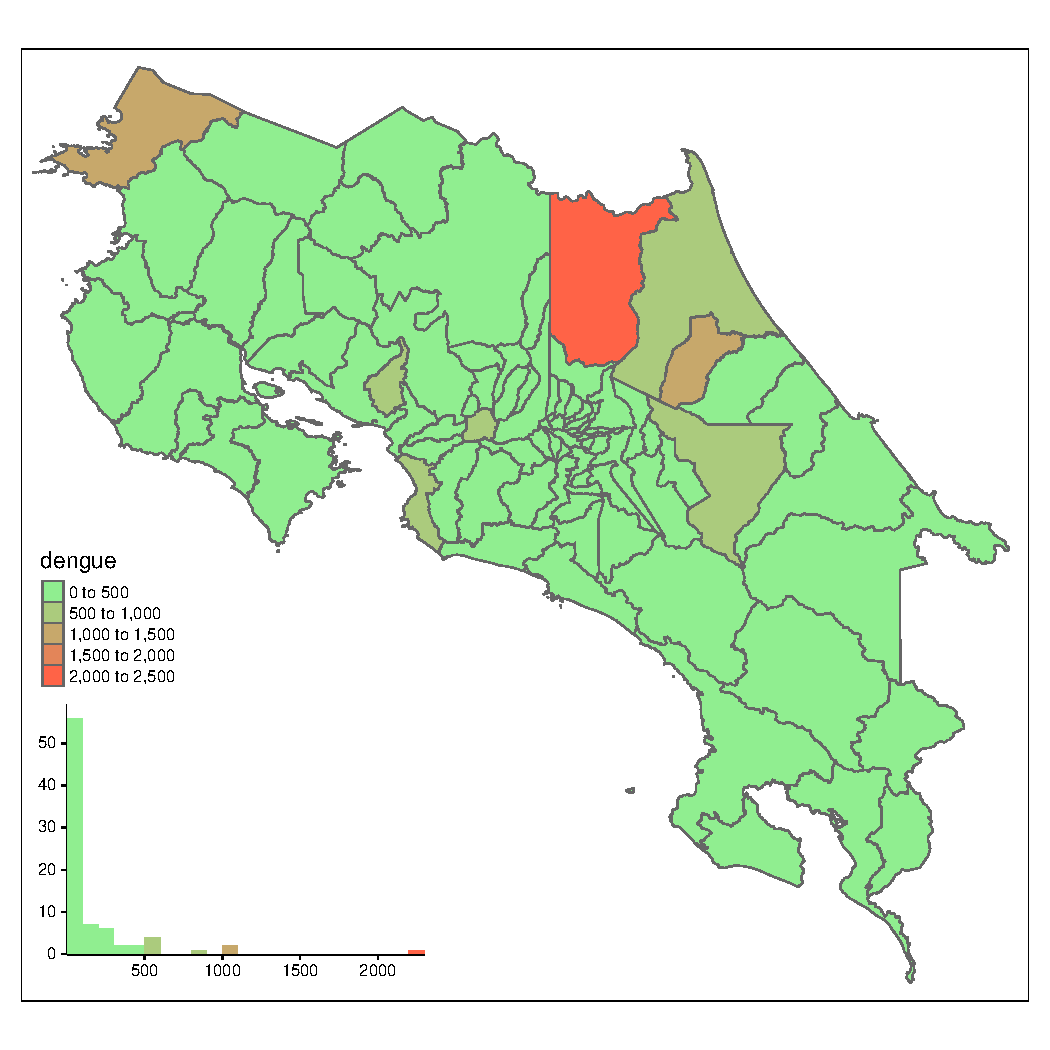
\includegraphics[width=.48\textwidth]{F11.pdf}
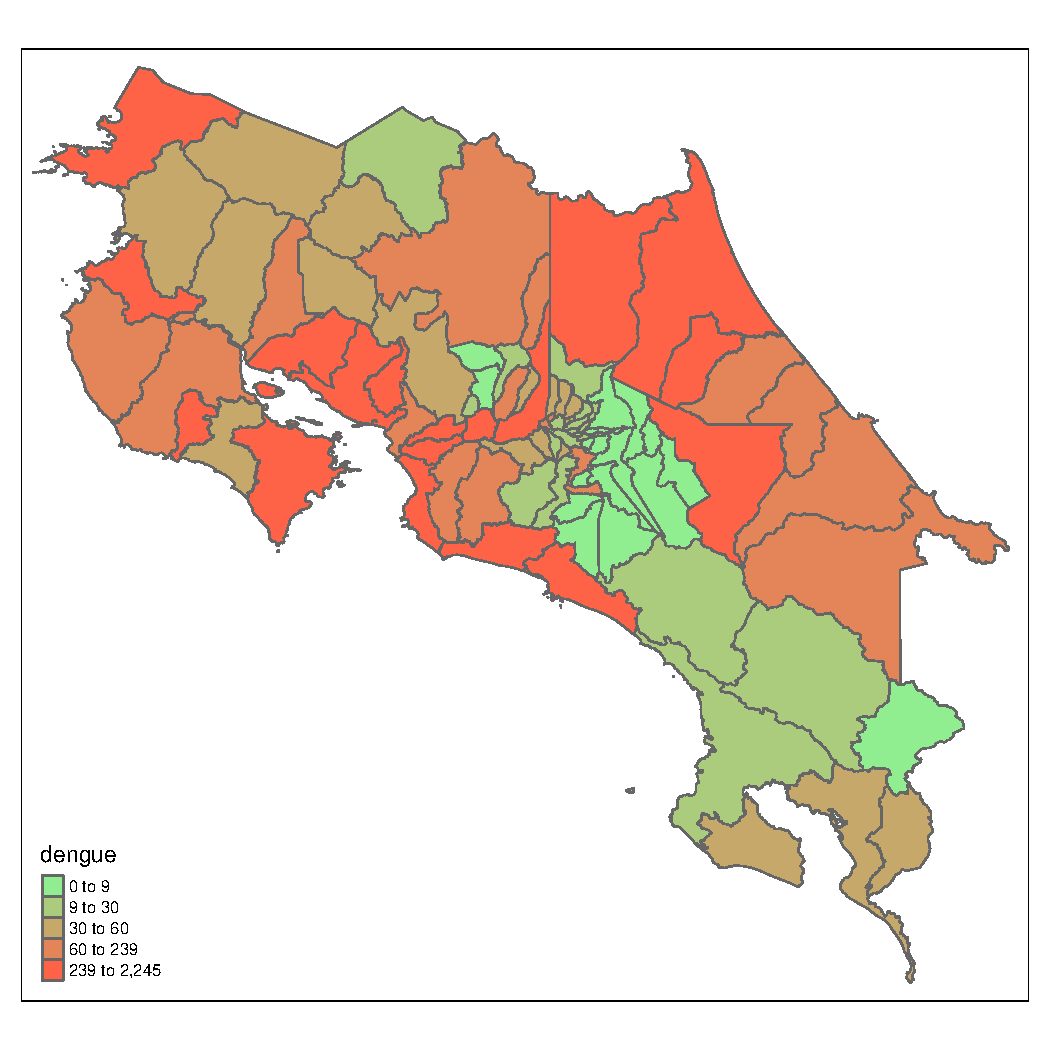
\includegraphics[width=.48\textwidth]{F12.pdf}
\caption{Tasa de dengue (100.000 habitantes) por cantón y tasa de dengue en quintiles por cantón, 2019.}
\end{figure}
\newpage
Se observa valores altos en los cantones específicos de Sarapiquí, La Cruz, Guácimo y Turrialba, además se incluye un histograma. Con este último gráfico se observa la distribución asimétrica positiva de la tasa de dengue, con un valor extremo muy marcado (Sarapiquí) con una tasa de dengue que sobrepasa los 2.000 por cada 100.000 habitantes, razón por la cual se tiene que mitigar este efecto con un mapa de la tasa de dengue por quintiles, que es el segundo mapa de la primera figura. En ese mapa se presenta una situación similar al primero, tasas elevadas en la región noroeste del país junto con regiones costeras del suroeste. En los anexos se incluyen mapas referidos a los casos de dengue y otra sigura que trata de minimizar el efecto del valor extremo mediante el uso de desviaciones estándar.
\newline
La figura 8 en la sección de anexos presenta la distribución espacial de las covariables utilizadas en el artículo. Dentro de las características más importantes se tiene: porcentajes altos en las zonas de Guanacaste y otras de Alajuela en cuanto a porcentaje de viviendas de tipo tugurio en el 2011, pocos cantones con alta densidad de la población, en la parte central del país  existe una mayor concentración de viviendas que eliminan los residuos sólidos por camión recolector, además las zonas de Guatuso y Upala tienen los porcentajes más bajos en esta variable. Por último en Heredia Puntarenas y Limón se concentran los porcentajes más bajos de viviendas con acueducto, información relevante es que los cantones de Talamanca y Sarapiquí poseen la mayor cantidad de viviendas sin acueducto.
\newline
Para la definición de la estructura de vecinos y la matriz de pesos, al no tener una referencia clara, se consideran varios métodos. En estructuras de vecinos, se trabajan los métodos de: reina, torre y vecinos más cercanos (Knn) considerando 2 vecinos y 4 vecinos. En la figura 2 se muestra el método de la reina y 4 vecinos más cercanos. Por otra parte, para la matriz de pesos se consideran las estructuras W, B y S, dando como resultado un total de 12 posibles combinaciones de vecinos y matriz de pesos. Se realiza la prueba de I de moran para cada una de estas combinaciones y los resultados se presentan en la tabla 1. Se concluye que la autocorrelación espacial está presente para cada una de las combinaciones, es decir, no importa cuál estructura de vecino se utilice y cómo se defina la matriz de pesos, la tasa de dengue en el 2019 posee autocorrelación espacial.
\begin{figure}[hbtp]
\centering
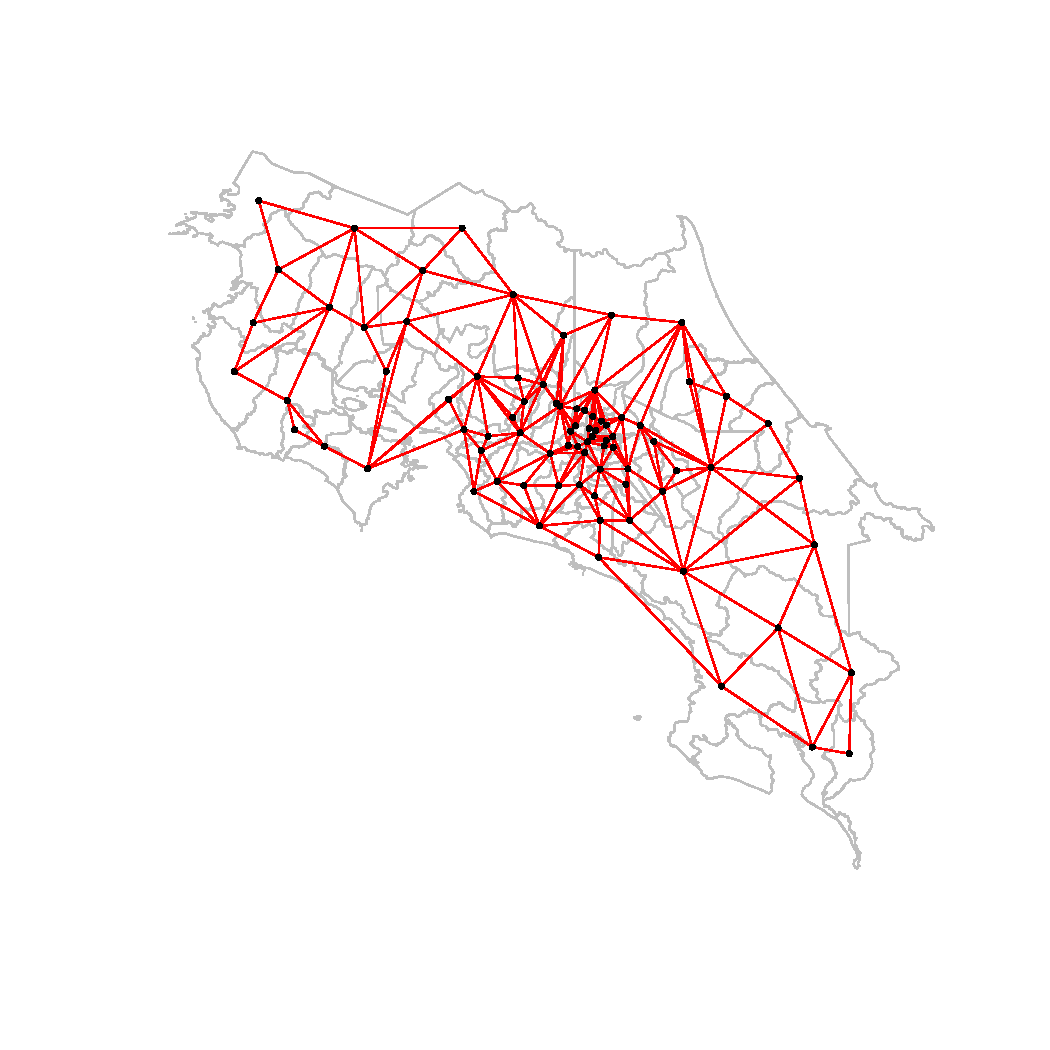
\includegraphics[width=.48\textwidth]{F21.pdf}
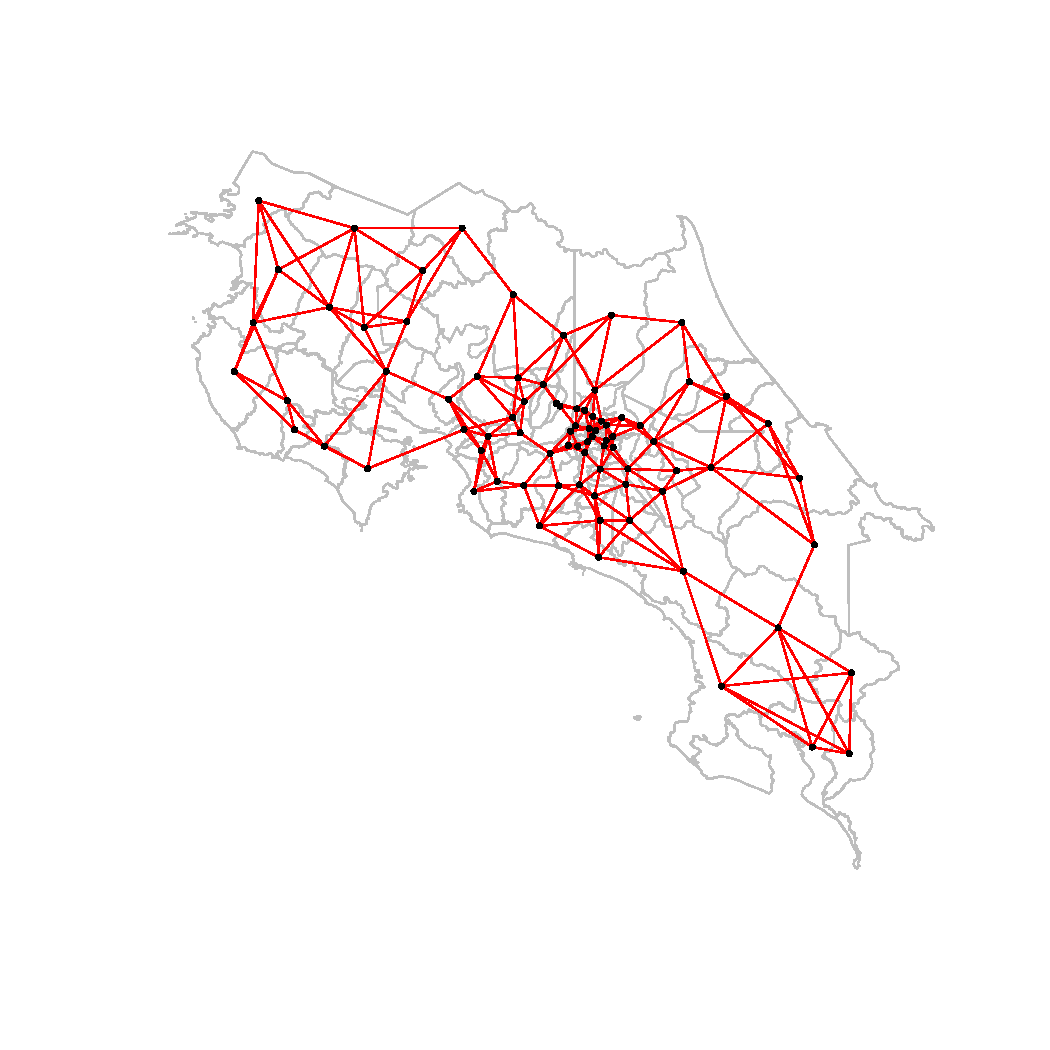
\includegraphics[width=.48\textwidth]{F22.pdf}
\caption{Estructuras de vecinos: Reina y Knn(4)}
\end{figure}

\begin{table}[h]
\centering
\caption{Valores-p para la prueba de autocorrelación espacial según la estrcutura de vecinos y la matriz de pesos}
\begin{tabular}{cccc}
\hline
\multirow{2}{*}{Vecinos} & \multicolumn{3}{l}{Matriz de pesos}\\ \cline{2-4} 
&W&B&S\\ \hline
Reina&0,009&0,007&0,006\\
Torre&0,011&0,008&0,008\\
Knn(2)&0,018&0,018&0,018\\
Knn(4)&0,026&0,026&0,026\\ \hline
\end{tabular}
\end{table}

Se realiza el estudio de los valores de influencia y los resultados se grafican en la figura 3. De esa figura cabe resaltar el comportamiento de la tasa de dengue junto con la tasa de dengue rezagada espacialmente, es decir, sus vecinos, que tienen una asociación lineal marcada por varios cantones que son valores de influencia y se ubican en el cuadrante alto-alto, mientras que solo un valor se ubica en el cuadrante bajo-bajo. Al realizar un mapa con estos valores se encuentran que los cantones del cuadrante alto-alto se ubican en la zona noroeste donde existe una agrupación bien definida. Mientras que el cantón de La Cruz de Guanacaste es el valor del cuadrante bajo-bajo. Para complementar esta información se realizan cuatro mapas de pruebas de Moran para cada supuesto en la tasa de dengue y el resultado se presenta en la figura 9 del anexo. A partir de este análisis se afirma la existencia de autocorrelación espacial y de agrupaciones espaciales en la tasa de dengue en la zona noroeste del país.

\begin{figure}[hbtp]
\centering
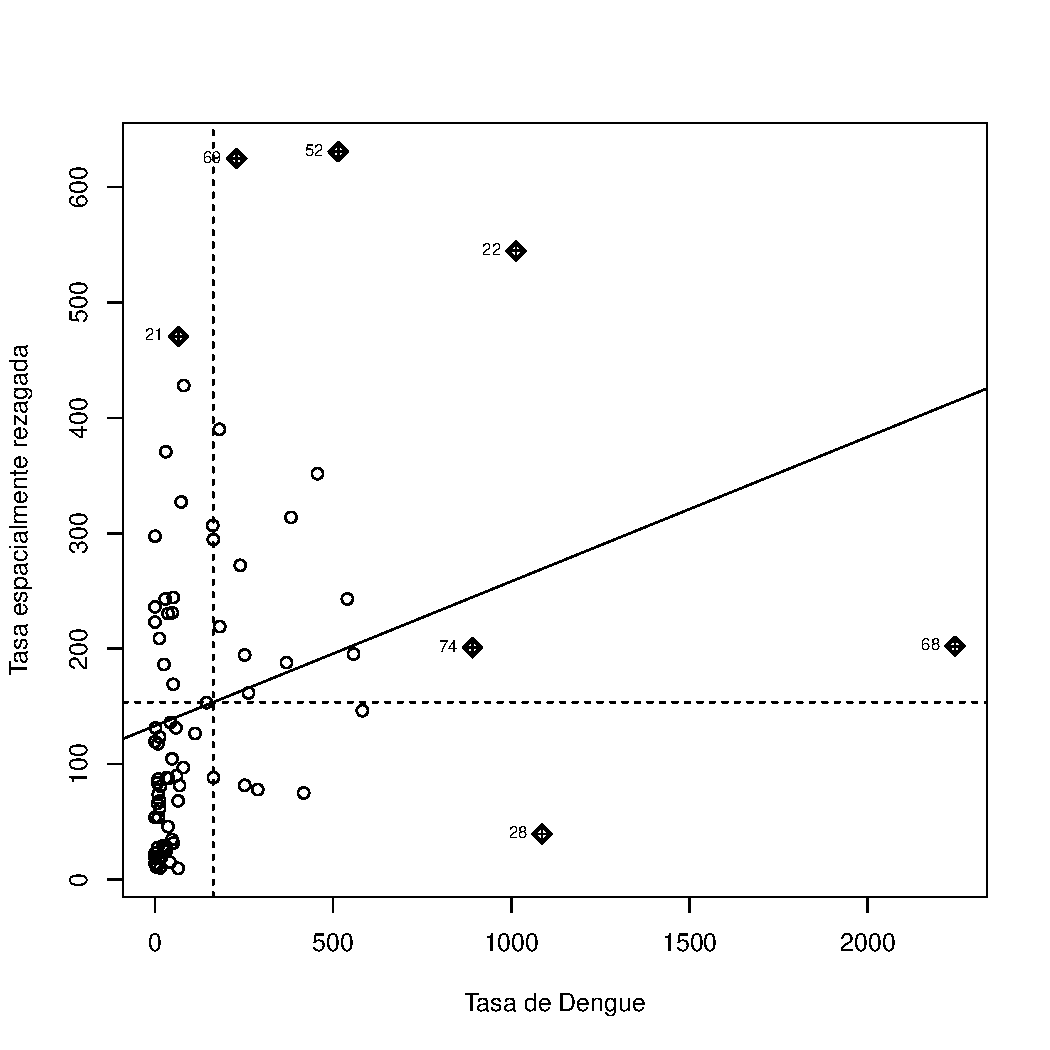
\includegraphics[width=.48\textwidth]{F31.pdf}
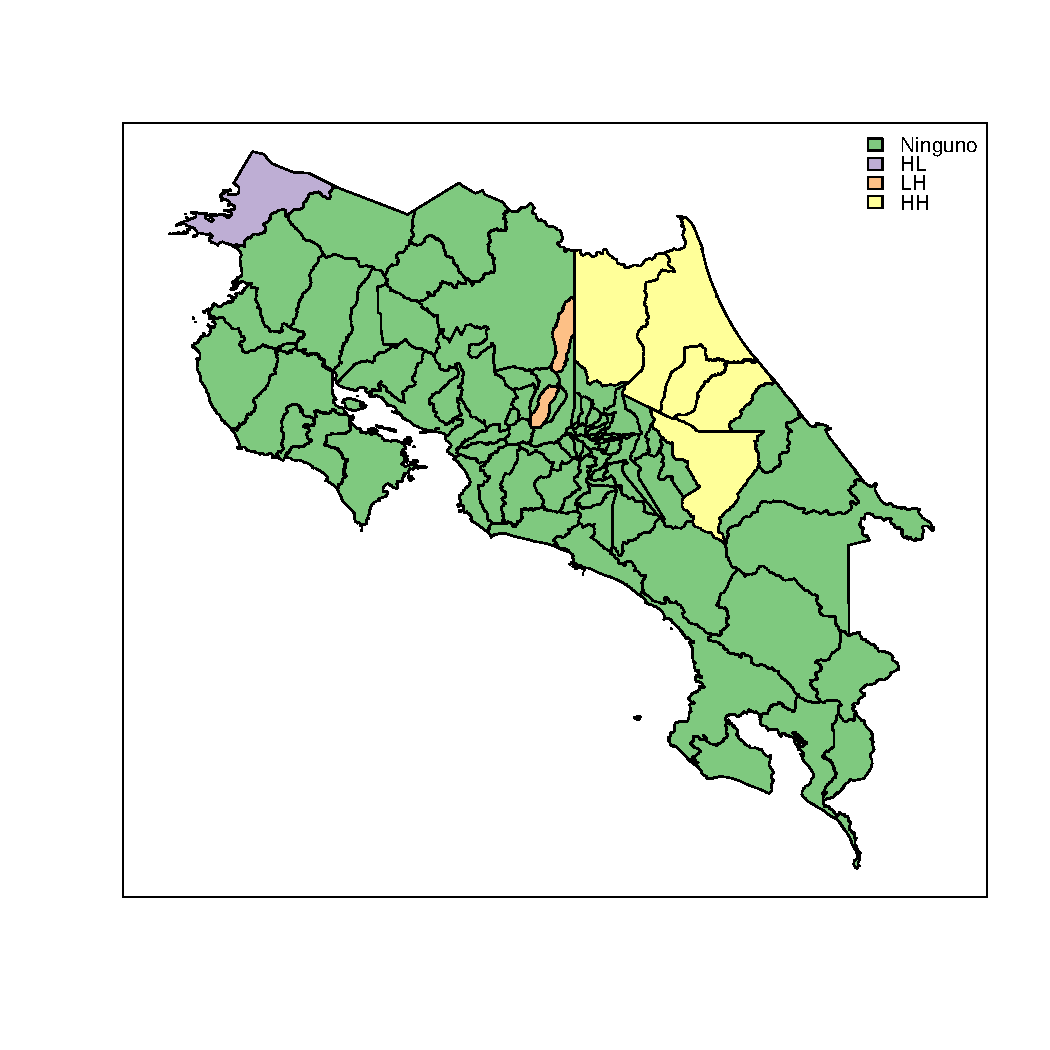
\includegraphics[width=.48\textwidth]{F32.pdf}
\caption{Casos de influencia}
\end{figure}

Por otro lado, se ajusta un modelo lineal (con tranformación raíz cuadrada en la variable respuesta) y dos modelos autoregresivos (\textit{SAR \& CAR}) que tratan de describir la tasa de dengue por 100.000 habitantes y un modelo lineal generalizado quasi-poisson con un término no paramétrico que trata de describir la cantidad de casos de dengue. Para cada uno de estos modelos se emplea el criterio AIC para determinar las covariables que resultan importantes para describir el fenómeno en cuestión. En los cuatro modelos las variables porcentaje de viviendas que eliminan los residuos sólidos por camión recolector y porcentaje de viviendas con acueducto resultan ser significativas al 5\% y minimizan el AIC en cada escenario. Este es un resultado esperado, pues se evidenció en el análsis descriptivo que estas variables presentan comportamiento similar a la tasa de dengue y a los casos de dengue en el 2019.
\newline
Los residuales de estos modelos se presentan en la figura 4, donde resalta que los dos modelos autoregresivos tienen problemas con el cantón de Sarapiquí y aledaños, mientras que los residuales de los  otros dos modelos son pequeños en comparación con los residuales de los modelos autoregresivos. Cabe destacar que al realizar la prueba de autocorrelación espacial para los residuales de cada uno de los cuatro modelos, solo los modelos autorregresivos no tienen rastro de componente de autocorrelación. Por otro lado, el modelo quasi-poisson con término no paramétrico de suavizamiento, explica aproximadamente el 88\% de la deviancia y posee un $R^{2}$ ajustado de 93\%, lo que quiere decir que un buen modelo para estos datos, sin embargo se sospecha un sobreajuste del término no paramétrico.

\begin{figure}[hbtp]
\centering
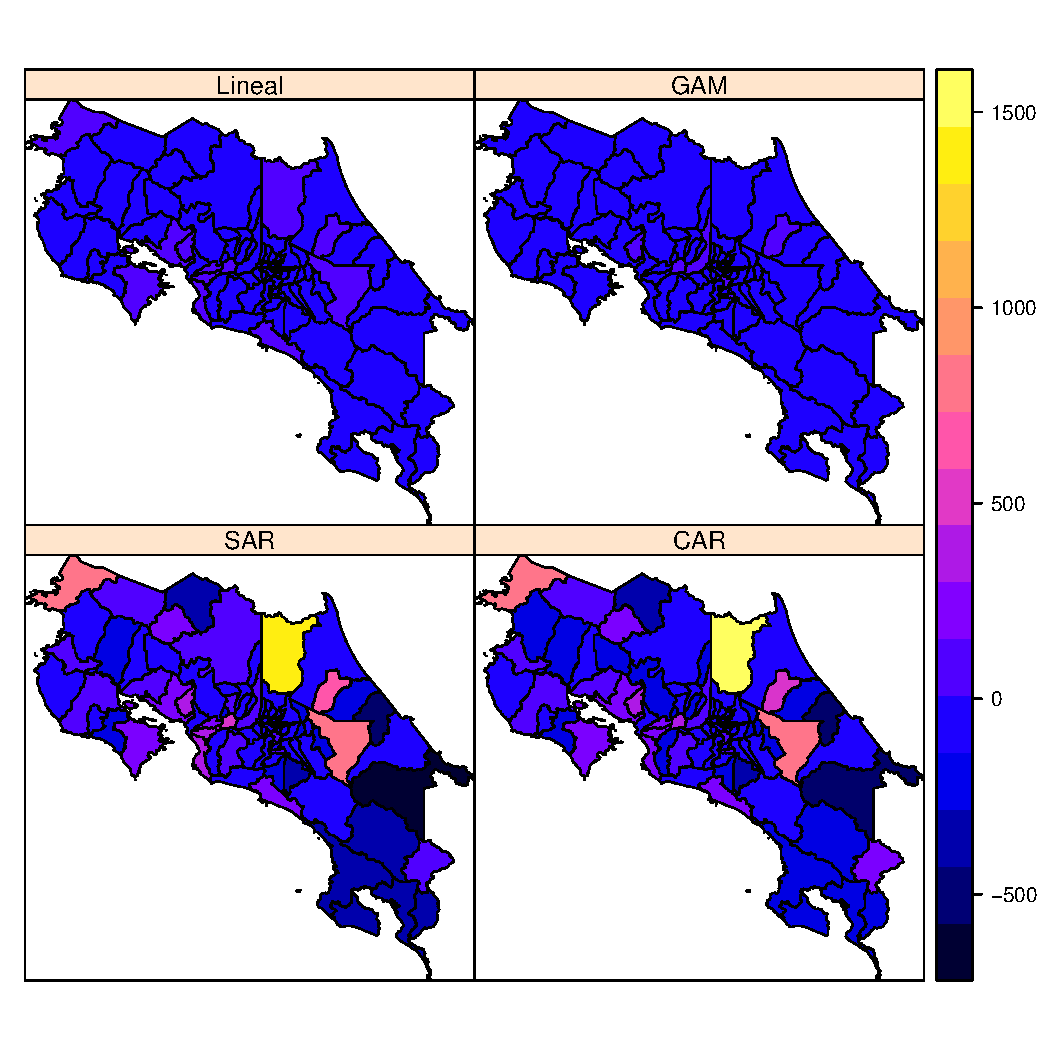
\includegraphics[scale=0.75]{F4.pdf}
\caption{Residuales de los cuatro modelos ajustados}
\end{figure}
Se concluye esta sección con un análisis epidemiológico del dengue. Para iniciar este último análisis se calcula y grafica los valores esperados en cada cantón, es decir, los valores que se esperarían observar si la disstribución de los casos del dengue fuera aleatoria. El contraste de este mapa con los observados se puede consultar en la figura 10 de la sección de anexos. En ese misma figura se observan las discrepancias entre los valores observados y esperados que, evidentemente, debería seguir el comportamiento de la densidad de la población. Se prosigue el análisis epidemiológico con el cálculo del riesgo relativo, o SMR (Standardised Mortality Ratio) \cite{sp} y su respectiva graficación en la figura 5, que además se completa con la figura 6, donde se muestran los intervalos de confianza del 95\% para el riesgo relativo de cada cantón.
\begin{figure}[hbtp]
\centering
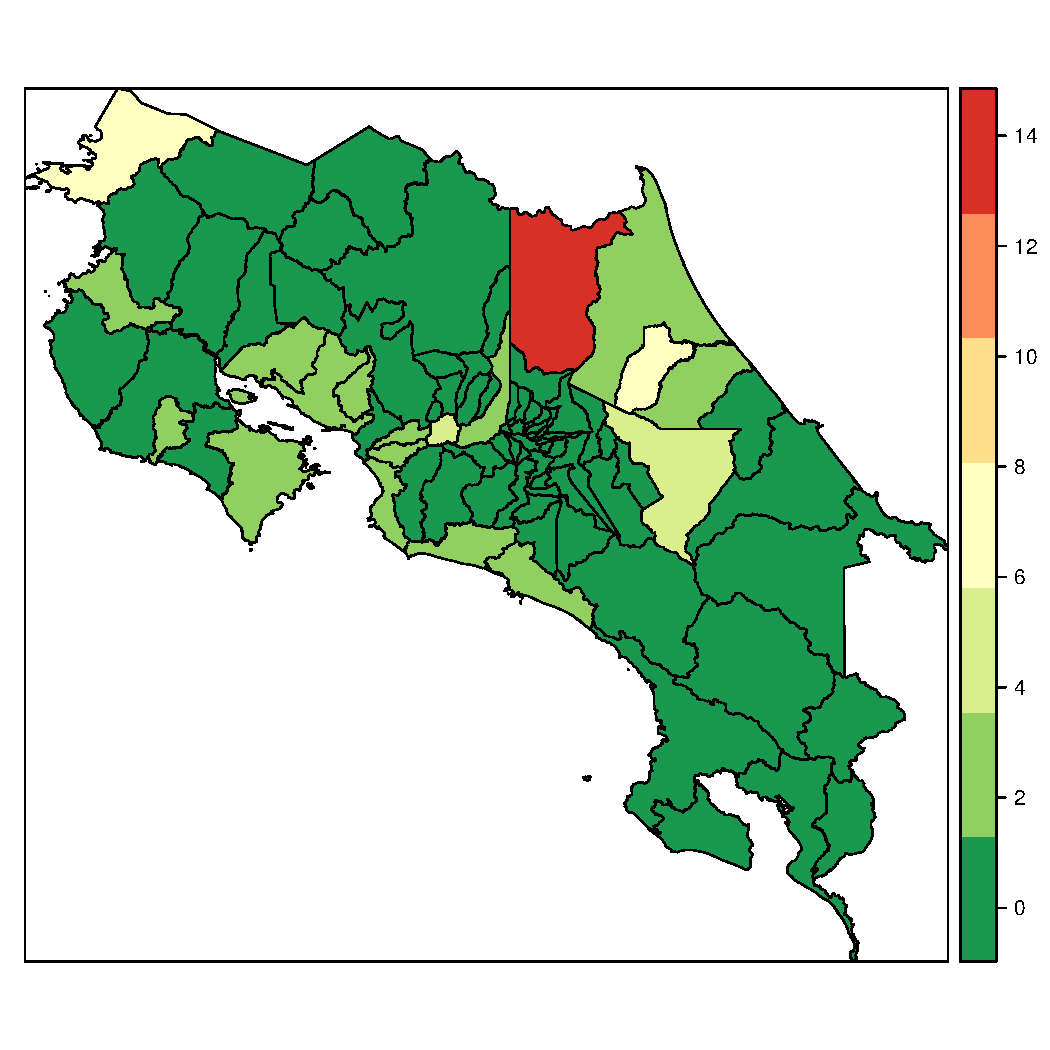
\includegraphics[scale=0.75]{F5.pdf}
\caption{Riesgo relativo}
\end{figure}

Aquí se destacan 8 cantones cuyo riesgo relativo resulta significativo: Sarapiquí, Guacimo, La Cruz, Turrialba, Atanas, Montes de Oro, Garabito y Pococí, es decir, una persona de Sarapiquí es hasta 22 veces más probable de enfermarse de dengue y una persona de Guácimo hasta 13 veces más probable. Se prosigue el análisis con un mapa de probabilidad de Choynowski, que muestra las probabilidades de las desviaciones observadas de la media calculado bajo el supuesto de que la distribución geográfica verdadera es uniforme y se presenta en la figura 11 del anexo. De la figura 11 se concluye que se podría centrar esfuerzos para prevenir los casos de dengue en los cantones de San Carlos, Limón y Talamanca, entre otros.
\newline
Finaliza esta sección con el cálculo de riesgos relativos mediante modelos empíricos bayesianos, específicamente se calculan 3 medidas: estimador empírico global de Bayes (mm), suavizado empírico de Bayes (ml) con parámetros $\nu = 0,255$ y $\alpha = 0,253$; y estimador empírico local de Bayes (mm.local). Los resultados se grafican en la figura 12 de Anexos. En general, estas medidas no difieren al cálculo del SMR.

\begin{figure}[h]
\centering
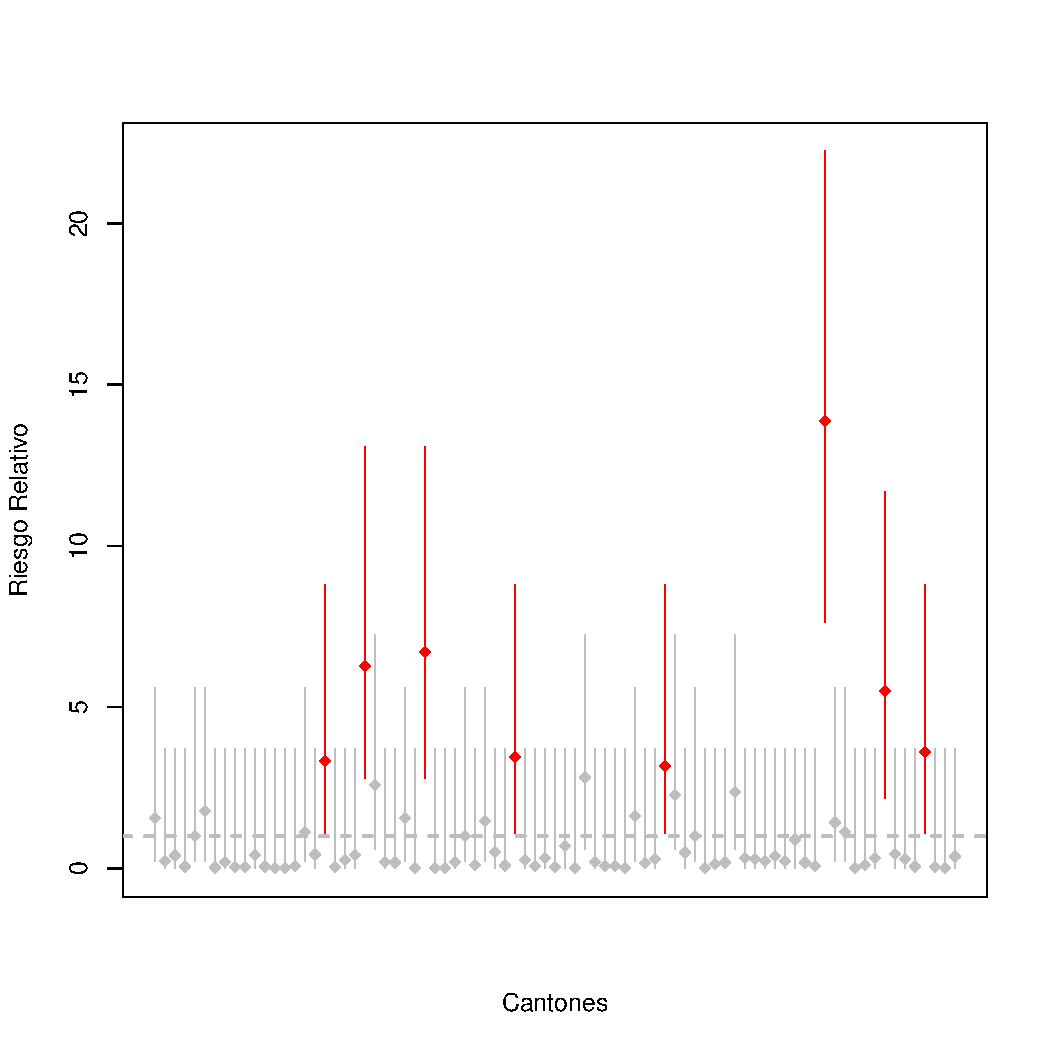
\includegraphics[scale=0.75]{F6.pdf}
\caption{Intervalos de confianza del 95\% para el riesgo relativo de dengue, por cantón.}
\end{figure}

\section{Conclusiones}

Por medio del análisis realizado se concluye que la ditribución de la tasa de dengue por 100.000 habitantes en el territorio de Costa Rica no es aleatoria, sino que existen patrones espaciales que se deben tomar en consideración, es decir, se evidenció la existencia de autocorrelación espacial. Además esta autocorrelación no depende de la estructura de vecinos ni de la selección de matriz de pesos que se elija, debido a que son muy evidenctes las agrupaciones espaciales que existen. También se determinó que la tasa de dengue por 100.000 habitantes puede ser explicada de gran forma mediante un modelo generalizado quasi-poisson con un término no paramétrico de suavizamiento y que las variables están asociadas a este fenómeno son el porcentaje de viviendas que eliminan los residuos sólidos por camión recolector y el porcentaje de viviendas con acueducto. Asimismo se sospecha de un sobreajuste del término no paramétrico de este modelo. Además que los habitantes de los cantones de Sarapiquí, Guacimo, La Cruz, Turrialba, Atanas, Montes de Oro, Garabito y Pococí tienen un riesgo mayor de contraer dengue y que se puede dedicar campañas de prevención en los cantones de San Carlos, Limón y Talamanca, entre otros. Por último los estimadores empíricos bayesianos no difieren mucho del SMR.
\newpage
\section{Anexos}

\begin{figure}[hbtp]
\centering
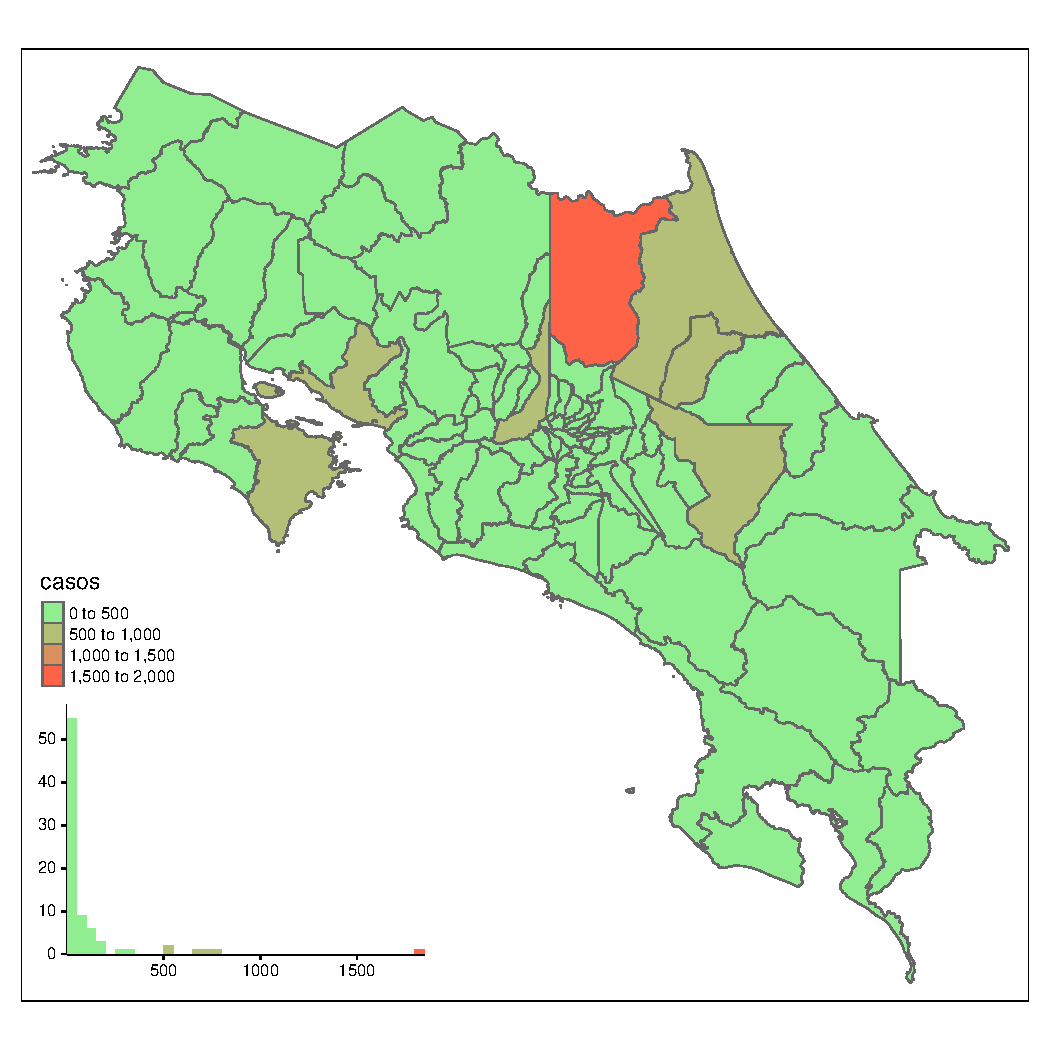
\includegraphics[width=.48\textwidth]{FA1.pdf}
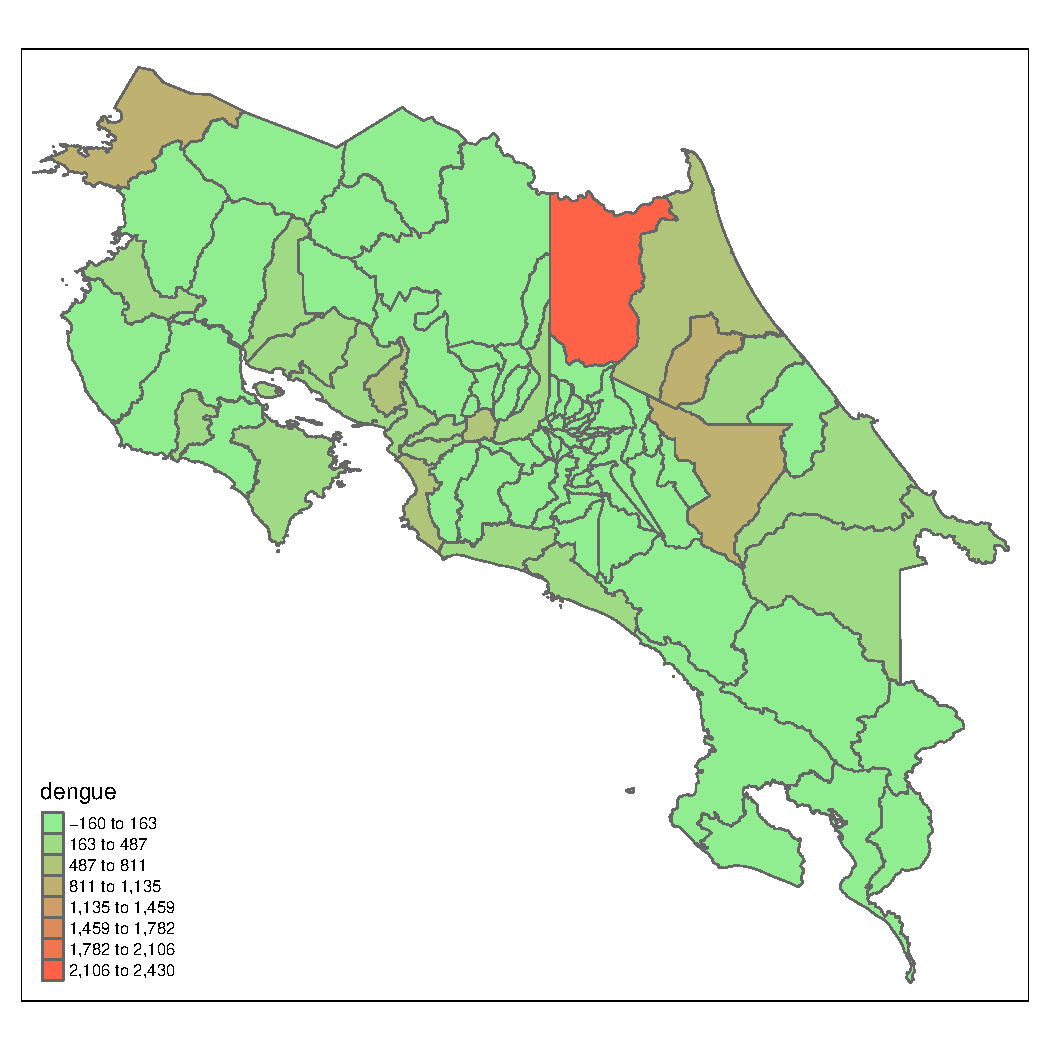
\includegraphics[width=.48\textwidth]{FA2.pdf}
\caption{Casos de dengue por cantón y desviación estándar de la tasa de dengue por 100.000 habitantes, 2019.}
\end{figure}
\newpage
\begin{figure}[hbtp]
\centering
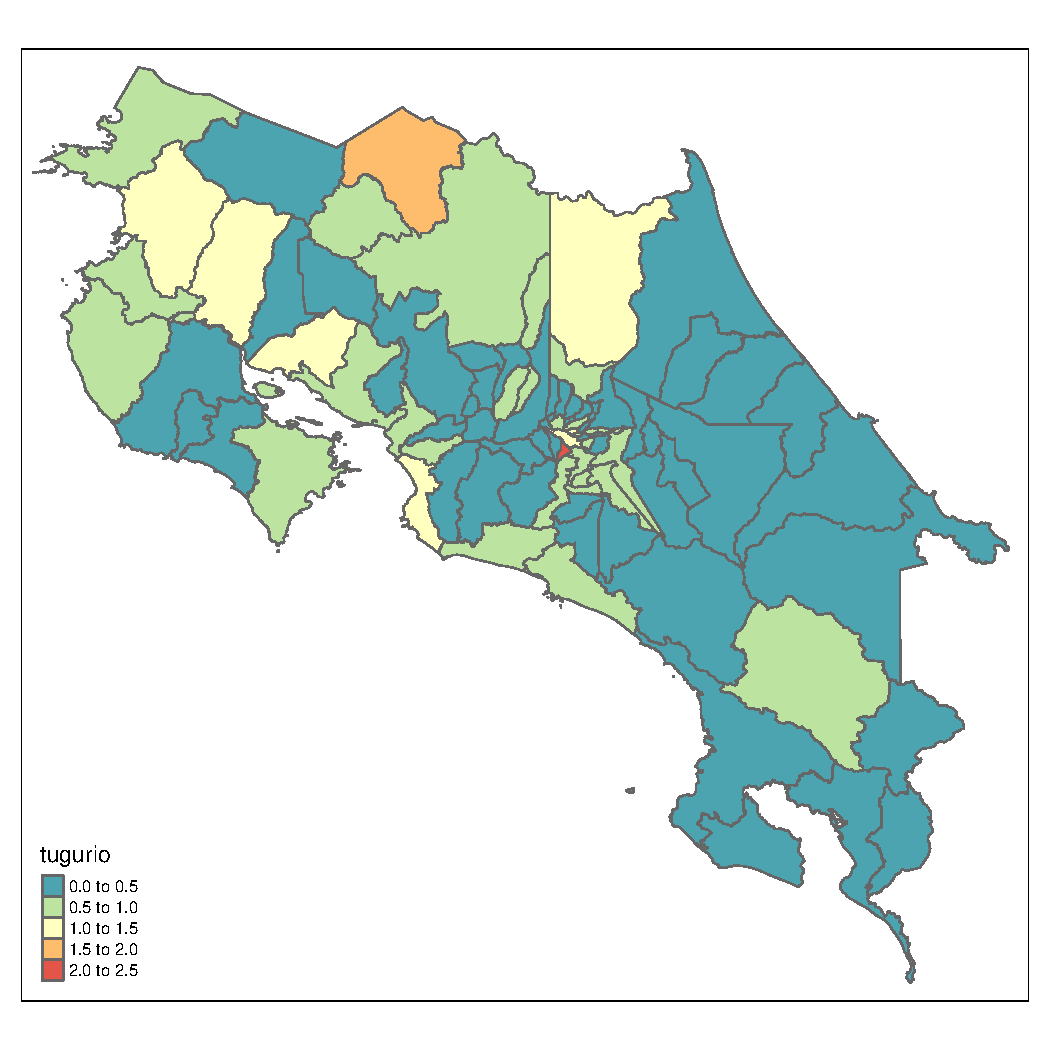
\includegraphics[width=.48\textwidth]{FA3.pdf}
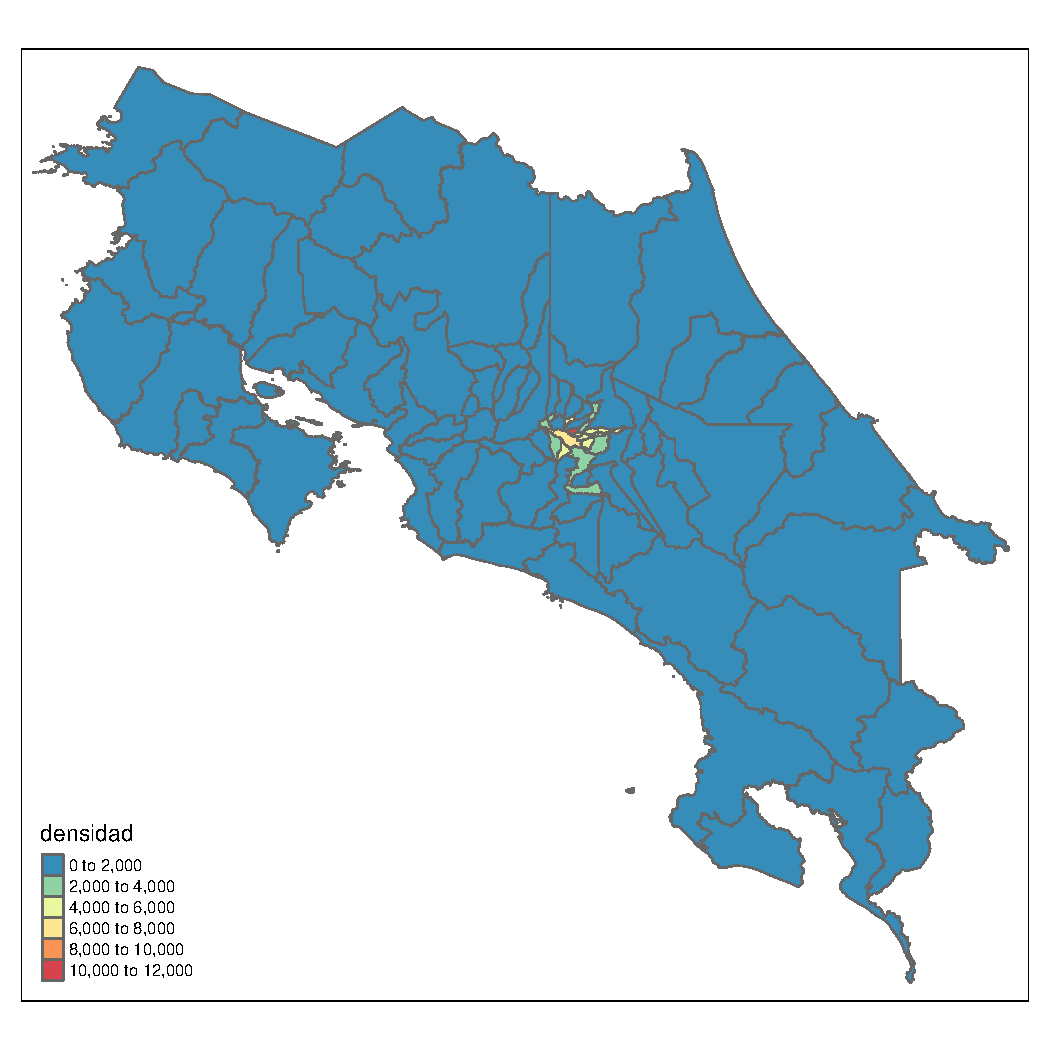
\includegraphics[width=.48\textwidth]{FA4.pdf}
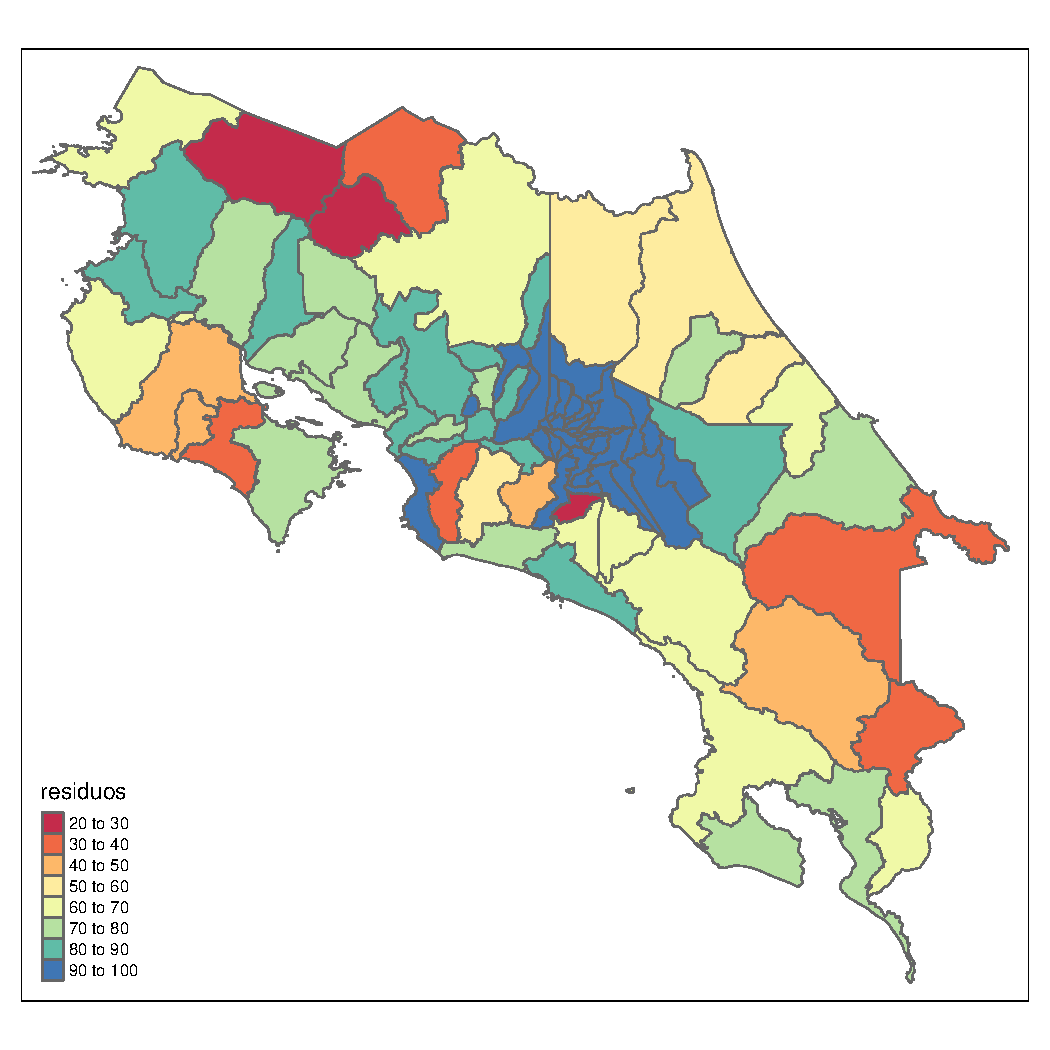
\includegraphics[width=.48\textwidth]{FA5.pdf}
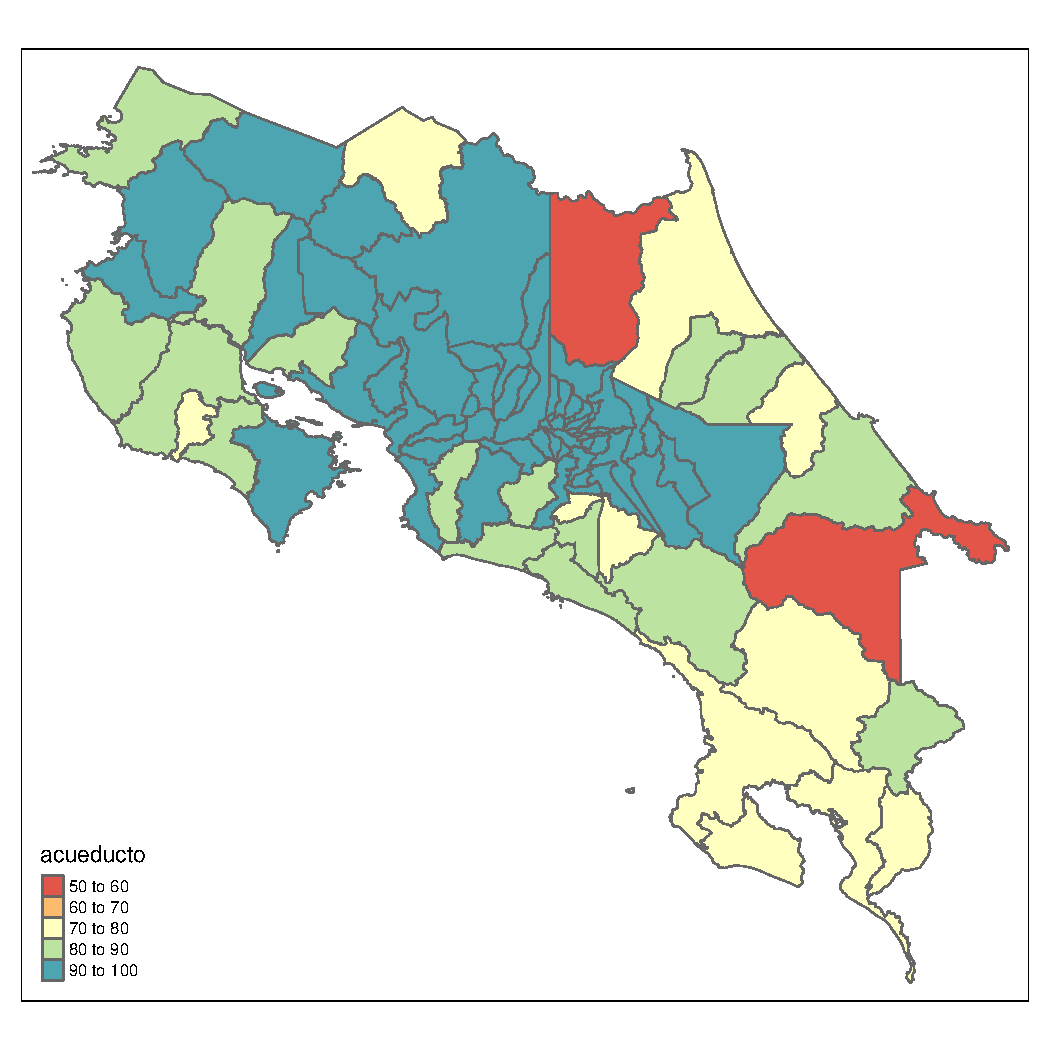
\includegraphics[width=.48\textwidth]{FA6.pdf}
\caption{Porcentaje de viviendas de tipo tugurio, densidad de la población, porcentaje de viviendas que eliminan los residuos sólidos por camión recolector, porcentaje de viviendas con acueducto}
\end{figure}
\newpage
\begin{figure}[hbtp]
\centering
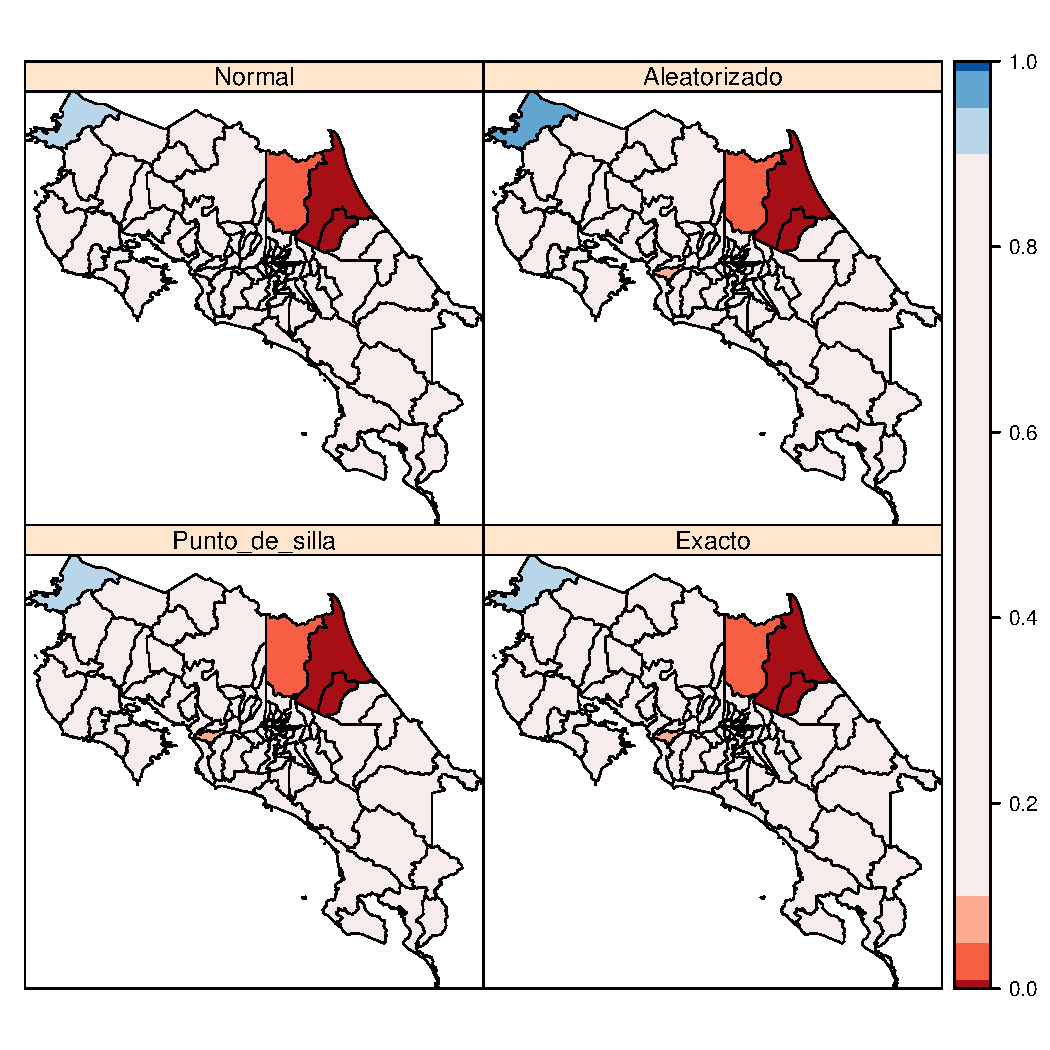
\includegraphics[scale=0.75]{FA7.pdf}
\caption{Probabilidad de cada supuesto en tasa de dengue por 100.000 habitantes}
\end{figure}
\newpage
\begin{figure}[hbtp]
\centering
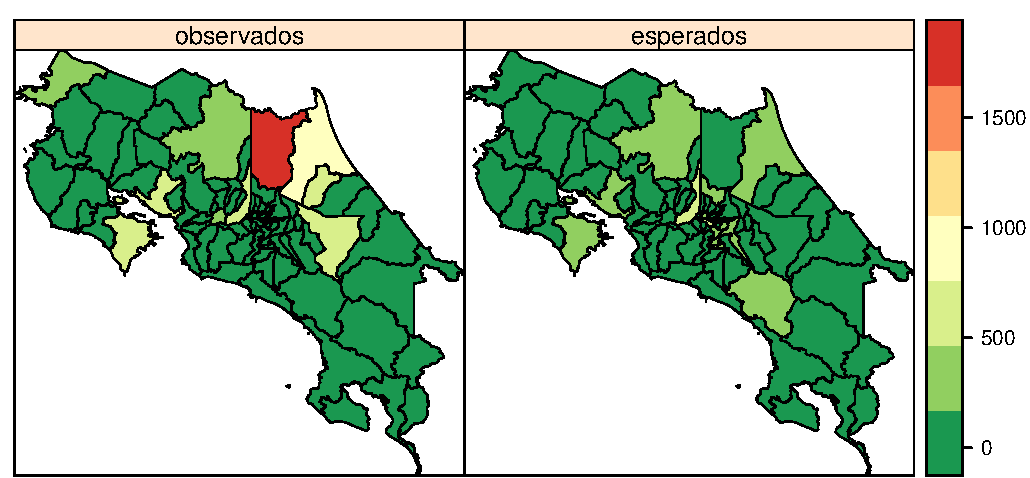
\includegraphics[scale=0.75]{FA8.pdf}
\caption{Valores observados y valores esperados de la tasa de dengue por 100.000 habitantes}
\end{figure}

\begin{figure}[hbtp]
\centering
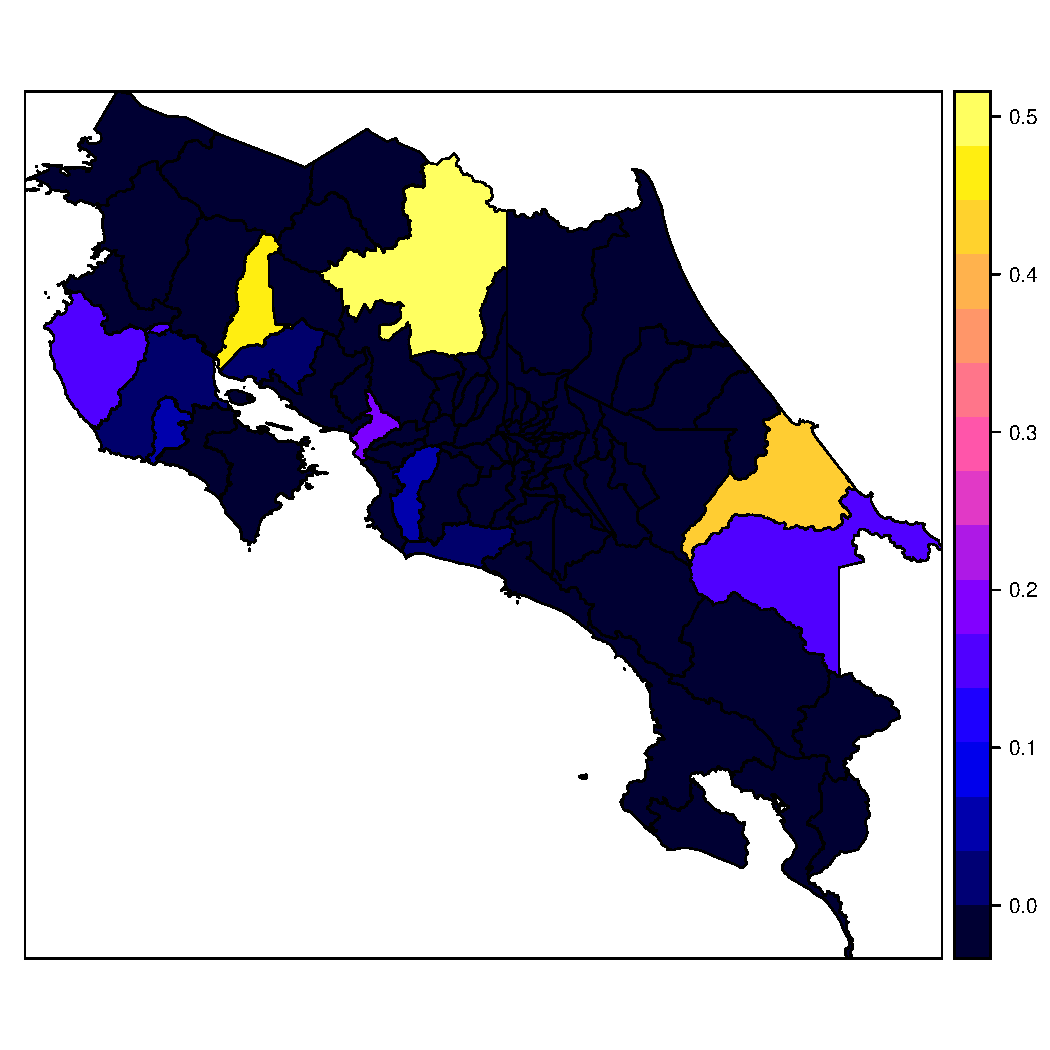
\includegraphics[scale=0.55]{FA9.pdf}
\caption{Mapa de probabilidad de Chownoysky}
\end{figure}
\newpage
\begin{figure}[hbtp]
\centering
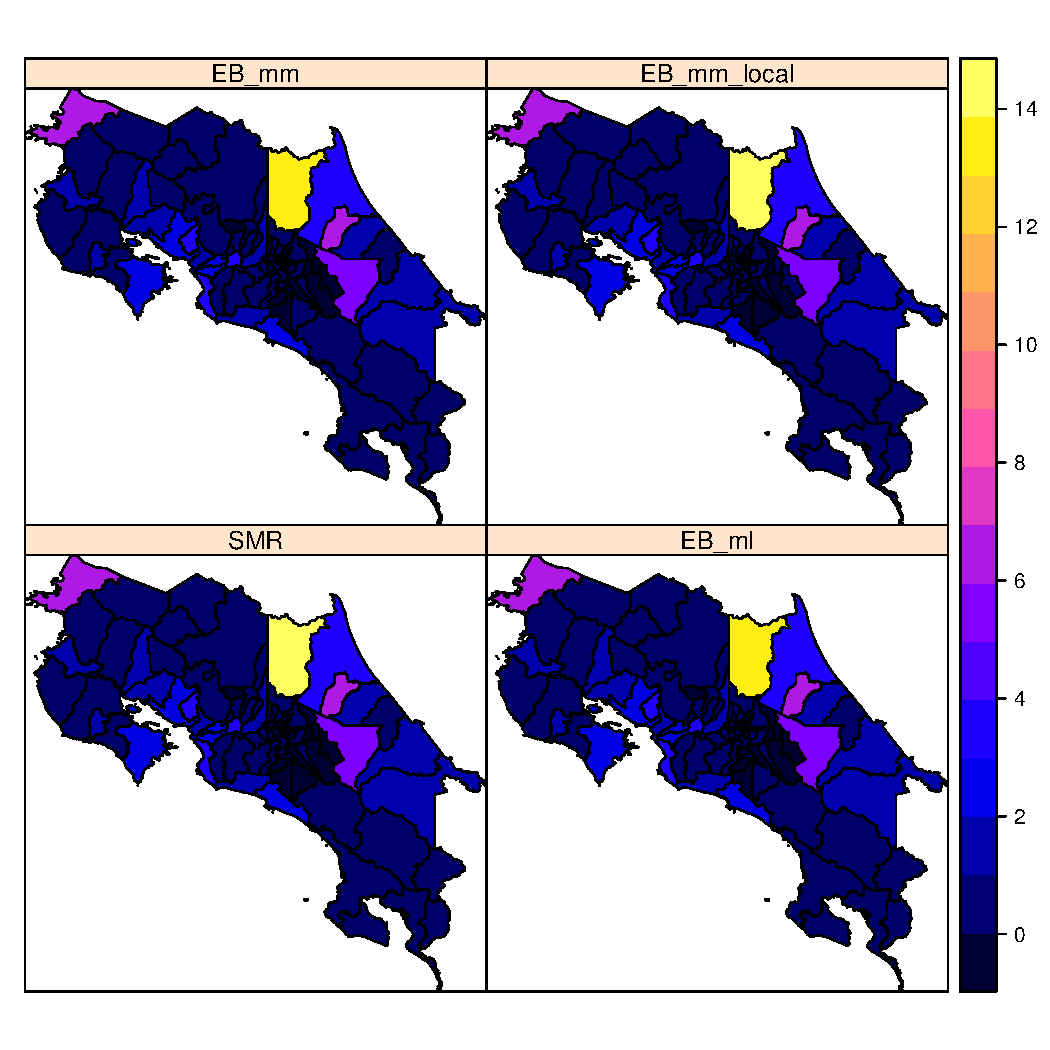
\includegraphics[scale=0.75]{FA10.pdf}
\caption{Estimador empírico global de Bayes (mm), Suavizado empírico de Bayes (ml) con parámetros $\nu = 0,255$ y $\alpha = 0,253$; estimador empírico local de Bayes (mm.local) y SMR}
\end{figure}
\newpage

%%Bibliografía
\bibliographystyle{apacite}
\bibliography{Referencias}
\end{document}


